\documentclass[t]{beamer}

% Load general definitions
% Preamble file - general definitions, package loading, etc.

%=================================
% Load packages
\usepackage{amssymb,amsmath}
\usepackage{graphicx}
\usepackage{url}
\usepackage{tikz}
\usetikzlibrary{mindmap,trees,arrows}
\usepackage{fancyvrb}
\usepackage[english]{babel}
\usepackage[latin1]{inputenc}
\usepackage{subfigure}
\usepackage{times}
\usepackage[T1]{fontenc}
\usepackage{cancel}
\usepackage{color}
\usepackage{listings}

%=================================
% Set mode
\mode<presentation>
{
	\usetheme{Madrid}
	\usecolortheme{whale}
	\useoutertheme{infolines}
	\setbeamercovered{invisible}
}

% Get rid of nav bar
\beamertemplatenavigationsymbolsempty

% Insert frame number at bottom of the page.
\usefoottemplate{\hfil\tiny{\color{black!90}\insertframenumber}} 

%=================================
% Define new commands

\newcommand\Real{{\mathbb{R}}}
%\newcommand{\vi}{\vspace{0.6\baselineskip}}
%\newcommand{\goodgap}{\hspace{\subfigtopskip}\hspace{\subfigbottomskip}}


% Equation environments
\newcommand{\beq}{\begin{equation}}
\newcommand{\eq}{\end{equation}}
\newcommand{\beqs}{\begin{equation*}}
\newcommand{\eqs}{\end{equation*}}
\newcommand{\beqn}{\begin{eqnarray}}
\newcommand{\eqn}{\end{eqnarray}}

% Bold variables
\newcommand{\mbf}[1]{\ensuremath{\mathbf{#1}}}

% Itemization
\newcommand{\bitem}{\begin{itemize}}
\newcommand{\eitem}{\end{itemize}}
\newcommand{\spitem}{\vskip 1em\item}
\newcommand{\bitems}{\begin{itemize}\item}
\newcommand{\benums}{\begin{enumerate}\item}
\newcommand{\eenum}{\end{enumerate}}

% color blocks
\newenvironment{colorblock}[2]{%
\setbeamercolor{block title}{#2}
\begin{block}{#1}}{\end{block}}

% Vertical spacing
\newcommand{\vone}{\vskip 1em}
\newcommand{\vhalf}{\vskip .5em}

% Frame environments
\newenvironment{ftst}[3][t]{%
\begin{frame}{environment=ftst,#1}
\frametitle{#2}
\framesubtitle{#3}}{\end{frame}}

\newenvironment{ftstf}[2]{
\begin{frame}[fragile,environment=ftstf]
\frametitle{#1}
\framesubtitle{#2}}{\end{frame}}

% colors
\definecolor{MyGray}{rgb}{0.5,0.5,0.5}
\definecolor{MyDBGray}{rgb}{0.1,0.1,0.4}
\definecolor{darkgreen}{rgb}{0,0.4,0}
\definecolor{black}{rgb}{0,0,0}
\def\defn#1{{\color{red} #1}}

% Footnote
\renewcommand{\thefootnote}{\alph{footnote}}

% Relaxed footnotes
\newcommand{\lfr}[1]{\let\thefootnote\relax\footnote{\tiny #1}}

% Verbatim environment - using FANCYVRB package
\DefineVerbatimEnvironment%
{rcode}{Verbatim}
{fontsize=\scriptsize}

% Verbatim environment - using LISTINGS package
%\lstnewenvironment{rcode} {\lstset{	language = R,
%									basicstyle = \scriptsize\ttfamily,
%									showspaces = false,
%									showstringspaces = false,
%									showtabs = false,
%									keywordstyle = \color{black}\bfseries,
%									commentstyle = \color{darkgreen},
%									numbers = none,
%									otherkeywords={	<-,
%													ggplot,
%													geom_boxplot,
%													facet_grid,
%													shapiro.test,
%													fligner.test,
%													glht,
%													with},
%									deletekeywords={data,
%													model,
%													residuals,
%													c,
%													axis,
%													default,
%													labels,
%													qq.text}}}%
%{}


% Specific definitions
\title[]{Design and Analysis of Experiments}
\subtitle[]{02 - The Role of Experimentation}
\author[]{Felipe Campelo\\{\footnotesize http://www.cpdee.ufmg.br/\textasciitilde fcampelo}}
\institute{Graduate Program in Electrical Engineering}
\date{\scriptsize Belo Horizonte\\March 2015}

\begin{document}

% cover page
\setbeamertemplate{footline}{}
\begin{frame}
\begin{flushright}

\includegraphics[width=.25\textwidth]{../figs/principal_completa3_ufmg}
\end{flushright}
  \titlepage
  \begin{tikzpicture}[remember picture,overlay]
  \node[anchor=south east,xshift=-5pt,yshift=122pt] at (current page.south east) {\tiny Version 2.11};
  \node[anchor=south west,yshift=0pt] at (current page.south west) {
\includegraphics[width=.15\textwidth]{../figs/by-nc-sa.png}};
  \end{tikzpicture}  
\end{frame}

%=====

% quotation page
  \begin{frame}[b]
		\frametitle{}
\begin{columns}[T]
\column{0.75\textwidth}
\flushright{\small ``\textit{There may be some beliefs that cannot be decided by\\
data, but such beliefs are dogmas that lie (double\\
entendre intended) beyond the reach of evidence.}''\\\ \\
John K. Kruschke\\
American mathematician and cognitive psychologist}
\column{0.25\textwidth}
\begin{tikzpicture}[remember picture,overlay]
\node[anchor=south east,yshift=30pt,xshift=0pt] at (current page.south east)
{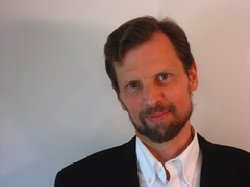
\includegraphics[width=\textwidth]{../figs/Kruschke.jpg}};
\end{tikzpicture}
\end{columns}
\vhalf
\lfr{Image: \url{http://www.amazon.com/John-K.-Kruschke/e/B00474BQRQ}}
\end{frame}

%=====

% Main slides
\begin{ftst}
{Experiments}
{Definition of experiment}
\vone
\begin{colorblock}{}{bg=green!30,fg=black}
\begin{center}
\textit{An experiment can be characterized as a test (or a series of tests) wherein changes are introduced in the state of a system or process, enabling the observation and characterization of effects that can occur as a result of these changes.}
\end{center}
\end{colorblock}
\vone
Usually performed with an objective in mind:

\bitems Uncovering influential variables in a given system or process;
	\spitem Determining desired values for certain parameters
	\spitem Characterize behavior of the system or process under study.
\eitem
\end{ftst}

%=====

\begin{ftst}
{Experiments}
{Data gathering}
\begin{block}{}
	{\small\bitems\alert{Retrospective study};
		\item Observational study;
		\item Designed experiment;
	\eitem}
\end{block}
\begin{block}{Characteristics}
	{\small\bitems Use of historical data;
	\item Investigating correlations;\eitem
	}
\end{block}
\begin{block}{Problems}
	{\small\bitems Data representativeness;
	\item Availability of data;\eitem
	}
\end{block}
\end{ftst}

%=====

\begin{ftst}
{Experiments}
{Data gathering}
\begin{block}{}
	{\small\bitems Retrospective study;
		\item \alert{Observational study};
		\item Designed experiment;
	\eitem}
\end{block}
\begin{block}{Characteristics}
	{\small\bitems Observation of the system with minimal disturbance;
	\item Investigation of usual behaviors;\eitem
	}
\end{block}
\begin{block}{Problems}
	{\small\bitems Low representativeness of extreme cases;
	\item Low variability can affect observation of interesting effects;\eitem
	}
\end{block}
\end{ftst}

%=====

\begin{ftst}
{Experiments}
{Data gathering}
\begin{block}{}
	{\small\bitems Retrospective study;
		\item Observational study;
		\item \alert{Designed experiment};
	\eitem}
\end{block}
\begin{block}{Characteristics}
	{\small\bitems Introduction of deliberate changes in the system;
		\item Inference on the \textit{causality} of the effects;
		\eitem}
\end{block}
\begin{block}{Problems}
	{\small\bitems Requires rigorous experimental design and data analysis;
	\item Usually more expensive.
	\eitem}
\end{block}
\end{ftst}

%=====

\begin{ftst}
{Experimentation strategies}
{Educated guessing}
\vspace{-1em}
\begin{columns}[T]
\column{1.02\textwidth}
	\begin{block}{}
		\bitems Select arbitrary combination of levels for the factors;
			\item Test and observe behavior; 
			\item Change one or two factors at a time, then re-test;
		\eitem
	\end{block}
\bitems Widely used in engineering;
\item Can achieve good results, but has a lot of limitations;
\eitem
\end{columns}
\end{ftst}


\begin{ftst}
{Experimentation strategies}
{Educated guessing}
\vspace{-1em}
\begin{columns}[T]
\column{0.8\textwidth}
	\begin{block}{}
		\bitems Select arbitrary combination;
			\item Test an observe; 
			\item Change and re-test;
		\eitem
	\end{block}
	\vone
	\centering
\includegraphics[width=0.65\textwidth]{../figs/edguess3.png}
\column{0.2\textwidth}
\vhalf
	\centering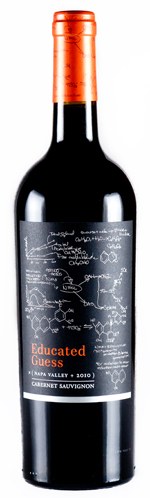
\includegraphics[width=.9\textwidth]{../figs/edguess2.jpg}
\end{columns}
\lfr{Images (c) Roots Run Deep Winery: \url{http://www.rootsrundeep.com/educated_guess.html}}
\end{ftst}

%=====

\begin{ftst}
{Experimentation strategies}
{Educated guessing}
\vspace{-1em}
\begin{columns}[T]
\column{0.8\textwidth}
	\begin{block}{}
		\bitems Select arbitrary combination;
			\item Test an observe; 
			\item Change and re-test;
		\eitem
	\end{block}
	\vone
	\centering
\includegraphics[width=0.65\textwidth]{../figs/edguess3.png}
\column{0.2\textwidth}
\vhalf
	\centering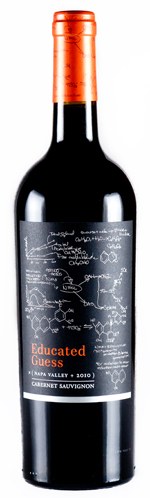
\includegraphics[width=.9\textwidth]{../figs/edguess2.jpg}
\end{columns}
\begin{tikzpicture}[remember picture,overlay]
	\node[anchor=south,yshift=20pt, xshift=-40pt] at (current page.south) {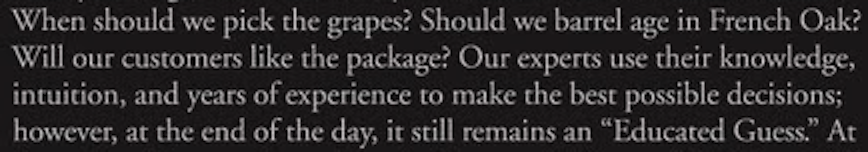
\includegraphics[width=9cm]{../figs/edguess3b.png}};
\end{tikzpicture}
\lfr{Images (c) Roots Run Deep Winery: \url{http://www.rootsrundeep.com/educated_guess.html}}
\end{ftst}

%=====

\begin{ftst}
{Experimentation strategies}
{COST: Change One Separate factor at a Time}
\begin{columns}[T]
\column{1.02\textwidth}
	\begin{block}{}
		\bitems Select a reference point;
			\item Change each factor individually, keeping all others constant;
		\eitem
	\end{block}
	\vone
	\bitems Widely used in practice;
		\item Can achieve good results as long as there are no interaction effects;
	\eitem
\end{columns}
\begin{tikzpicture}[remember picture,overlay]
	\node[anchor=south east,yshift=0pt, xshift=-5pt] at (current page.south east) {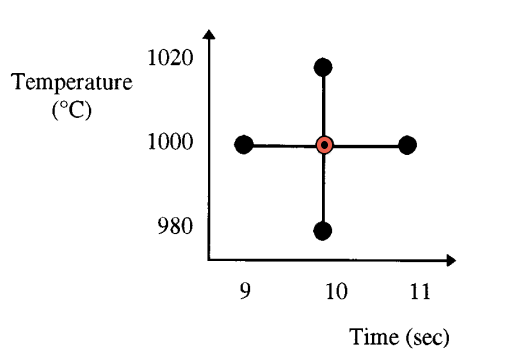
\includegraphics[width=5.5cm]{../figs/OFAT01c.png}};
\end{tikzpicture}
\lfr{Image: (c) D.C. Montgomery}
\end{ftst}

%=====

\begin{ftst}
{Experimentation strategies}
{Factorial designs}
\begin{columns}[T]
\column{1.02\textwidth}
	\begin{block}{}
		\bitems Select \textbf{levels} for each factor;
			\item Vary the factors simultaneously, in a systematic way;
		\eitem
	\end{block}
	\bitems Estimation of main effects and interactions;
		\item Greater precision in the effect estimates;
		\item More efficient use of resources (information/observation);
	\eitem
\end{columns}
\begin{tikzpicture}[remember picture,overlay]
	\node[anchor=south east,yshift=0pt, xshift=-5pt] at (current page.south east) {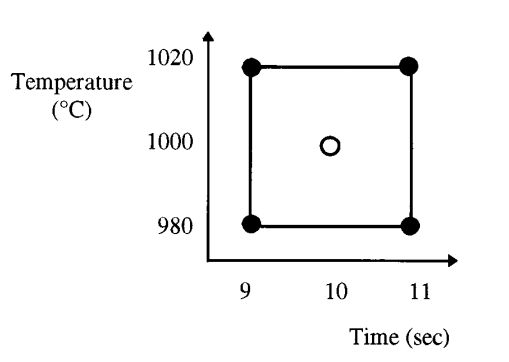
\includegraphics[width=5.5cm]{../figs/FFD01a.png}};
\end{tikzpicture}
\lfr{Image: (c) D.C. Montgomery}
\end{ftst}

%=====

\begin{ftst}
{Fundamental principles}
{Design of experiments (DoE)}
\vone
\begin{colorblock}{}{bg=green!30,fg=black}
\begin{center}
\textit{Process of designing data gathering protocols to enable\\
accurate analyses by statistical tools, capable of supporting\\
sound and objective conclusions.}
\end{center}
\end{colorblock}

\bitems Applicable to systems and processes subject to noise, experimental errors, uncertainties, etc.
	\item Necessary for the conclusions to have a quantifiable meaning;
	\item Helpful in avoiding errors due to personal biases or other artifacts of experimentation and analysis.
\eitem
\end{ftst}

%=====

\begin{ftst}
{Fundamental principles}
{Design of experiments (DoE)}
\begin{block}{Design of the experiment}
	\small
	\bitems Scientific/technical question of interest;
		\item Selection of variables and values;
		\item Definition of the desired confidence level;
		\item Sample size calculations;
		\item Determination of protocols for data gathering;
	\eitem
\end{block}
\begin{block}{Statistical analyses of the data}
	\small
	\bitems Calculation of a test statistic;
		\item Validation of the assumptions of the statistical model;
		\item Calculation of the magnitude of effects;
		\item Drawing of conclusions and recommendations;
	\eitem
\end{block}
\end{ftst}

%=====

\begin{ftst}
{Fundamental principles}
{Design of experiments (DoE)}
\begin{block}{}
	\bitems \alert{Repetition and replication};
		\item Randomization;
		\item Blocking.
	\eitem
\end{block}
	\bitems Repeated measurements - estimation of within-group variability;
		\item Replication - estimative of the experimental error;
		\item Greater precision in estimating the model parameters;
	\eitem
\end{ftst}

%=====

\begin{ftst}
{Fundamental principles}
{Design of experiments (DoE)}
\begin{block}{}
	\bitems Repetition and replication;
		\item \alert{Randomization};
		\item Blocking;
	\eitem
\end{block}
\bitems Avoids contamination of the data by order-dependent effects such as:

	\bitems Heating effects;
		\spitem Wear and tear effects;
		\spitem External interferences;
	\eitem
\eitem
\end{ftst}

%=====

\begin{ftst}
{Fundamental principles}
{Design of experiments (DoE)}
\begin{block}{}
	\bitems Repetition and replication;
		\item Randomization;
		\item \alert{Blocking};
	\eitem
\end{block}
\bitems Isolation of nuisance variables (those that influence the response, but are not interesting for the analyses) that can be controlled;
	\spitem Improvement in the estimation of effects for the factors of interest;
	\spitem Reduction or eliminations of inconvenient factor effects;
\eitem
\end{ftst}

%=====

\begin{ftst}
{Fundamental principles}
{The role of experimental design}
Experimental design is useful for avoiding the influence of spurious factors and personal biases on the results, by performing experiments in a impartial and objective way.
\begin{colorblock}{}{bg=green!30,fg=black}
	\vhalf
	\centering``\textit{Never have too much love for your hypotheses.}''
	\vspace{0.5em}
\end{colorblock}
\vone
\begin{columns}[T] 
\column{0.7\textwidth}
	\begin{colorblock}{}{bg=green!30,fg=black}
		\flushright{``\textit{The great tragedy of Science - the slaying of a\\
		\vspace{-1em}\flushright beautiful hypothesis by an ugly fact.}''\\
		-- Thomas H. Huxley}
		\vspace{0.5em}
	\end{colorblock}
\column{0.3\textwidth}
\end{columns}
\begin{tikzpicture}[remember picture,overlay]
	\node[anchor=south east,yshift=20pt, xshift=-10pt] at (current page.south east) {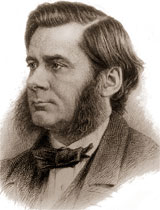
\includegraphics[width=2.5cm]{../figs/huxley.png}};
\end{tikzpicture}
\lfr{Image: \url{http://www.iep.utm.edu/huxley/}}
\end{ftst}

%=====

\begin{ftst}
{Example}
{Jacques Benveniste and the memory of water}
\begin{columns}
\column[T]{0.85\textwidth}
	\bitems Nature (1988);
		\item Investigation committee: Maddox, Stewart, Randi;
		\item Retracted by Nature due to evidence of misconduct.
	\eitem
\column[T]{0.15\textwidth}
	\begin{tikzpicture}[remember picture,overlay]
		\node[anchor=north east,yshift=-50pt, xshift=-10pt] at (current page.north east) {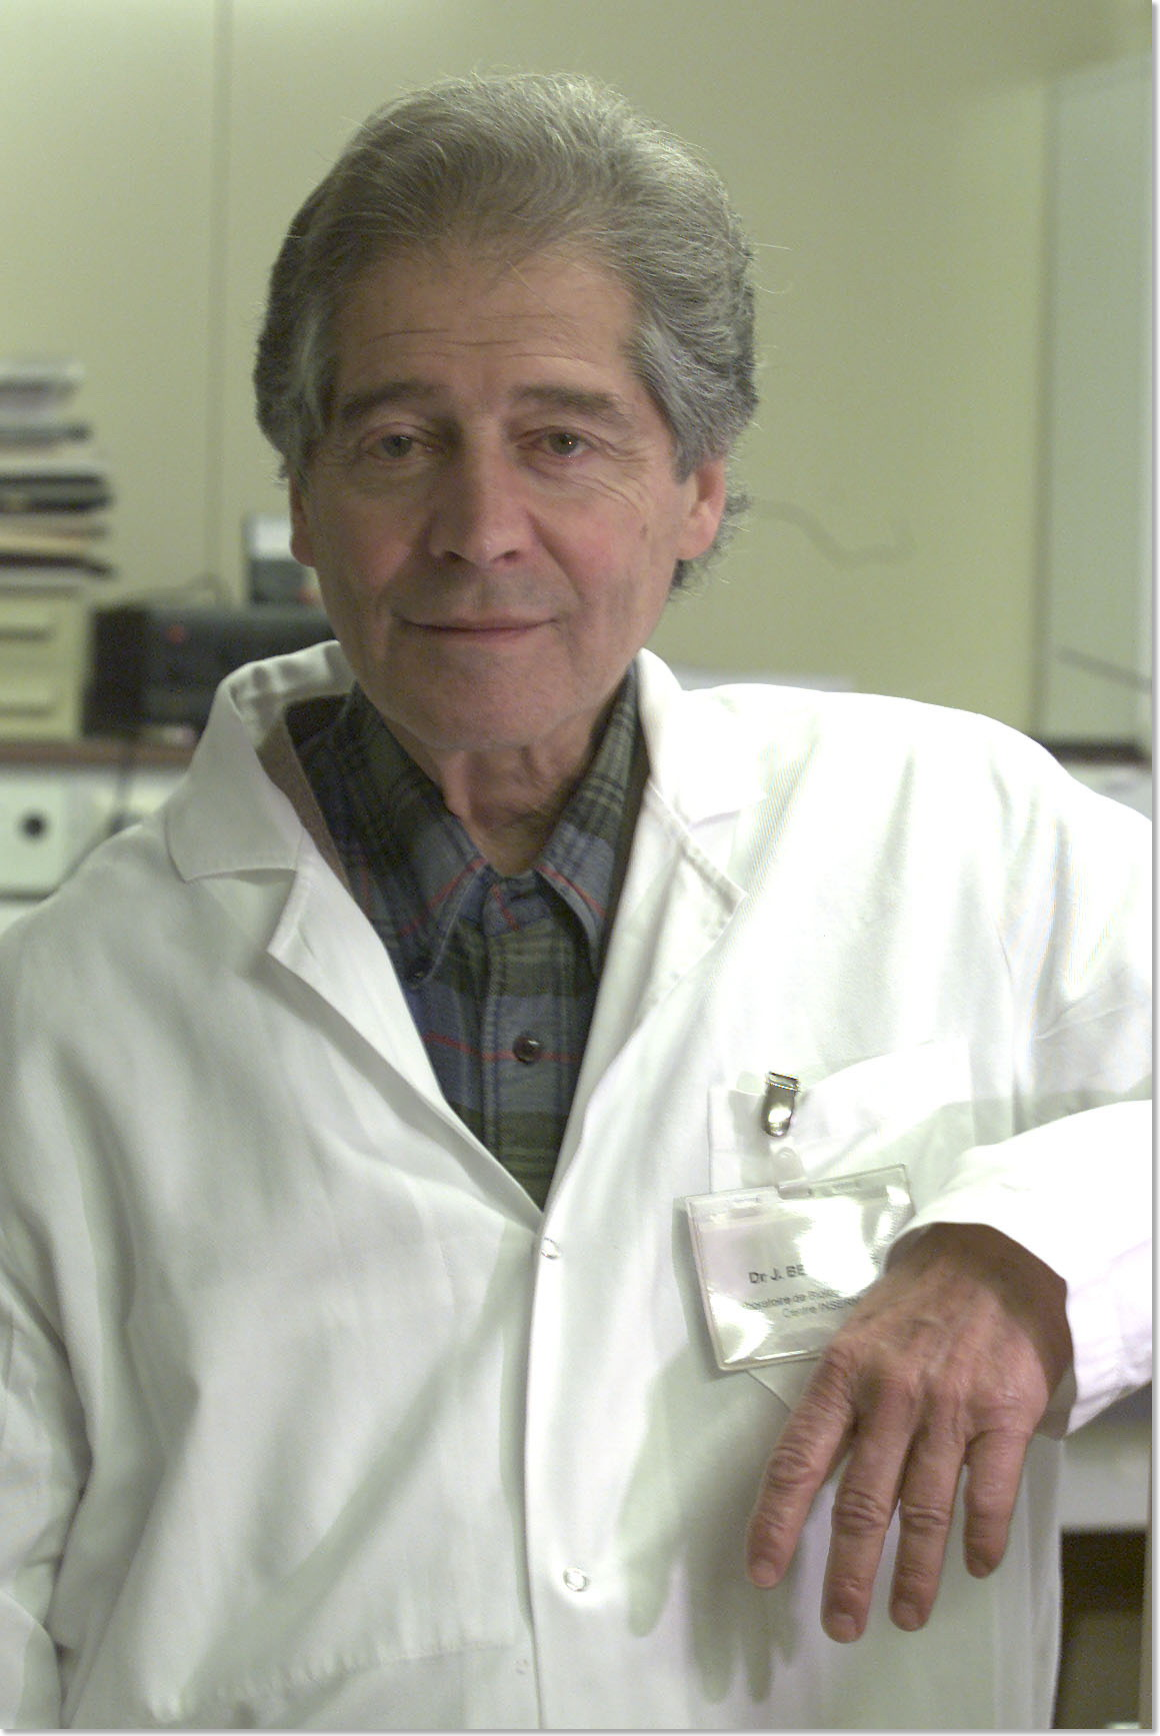
\includegraphics[width=1.1\textwidth]{../figs/benveniste.png}};
	\end{tikzpicture}
\end{columns}
\vone
\begin{columns}
\column[T]{0.8\textwidth}
	\begin{block}{Methodological problems}
	\small
	\bitems Experimenter bias (absence of proper blinding);
		\item Cherrypicking (selective recording of results);
		\item Unaccounted sampling errors;
		\item Possible contamination;
		\item Complete lack of prior physical/ chemical plausibility;
		\item \textbf{Non-reproducibility}.
	\eitem
\end{block}
\column[T]{0.2\textwidth}
\end{columns}
\lfr{Image: \url{http://www.jacques-benveniste.org/inmemoriam/photo1.html}}
\end{ftst}

%=====

\begin{ftst}
{Structure of Experimental Design}
{Main points}
To enable the use of a scientific approach in the design of an experiment, it is important to have on a solid understanding of:
\vhalf
\bitems The field where the experiment is to be conducted;
	\spitem The strategy for data collection;
	\spitem The way the data should be analyzed (at least qualitatively).
\eitem
\end{ftst}

%=====

\begin{ftst}
{Structure of Experimental Design}
{Guidelines for a good design}
\bitems Pre-experimental design:

	\bitems Identification and definition of the problem;
		\spitem Selection of experimental and response variables of interest;
		\spitem Choice of experimental protocols;
	\eitem
	\spitem Choice of the experimental design;
	\spitem Collection of the data;
	\spitem Statistical data analyses;
	\spitem Conclusions and recommendations;
\eitem
\end{ftst}

%=====

\begin{ftst}
{Pre-experimental design}
{Before we start}
\bitems Is the investigation relevant?
	\spitem Would the results be interesting for the research community?
	\spitem Practical relevance?
	\bitems Employ exploratory experiments;\eitem
	\spitem Placement within the literature;
	\bitems Avoid repetition and irrelevance.\eitem
\eitem
\begin{columns}[T]
\column{0.7\textwidth}
\begin{colorblock}{}{bg=green!30,fg=black}
{\ \\\ \\\scriptsize``\textit{Sometimes one should do a completely wild experiment,\\like blowing the trumpet to the tulips every morning\\for a month. Probably nothing would happen, but what if it did?}''\\}
{\tiny -- Sir George Howard Darwin}
\end{colorblock}
\column{0.3\textwidth}
\end{columns}
\begin{tikzpicture} [remember picture,overlay]
\node[anchor=south east,yshift=0pt,xshift=10pt] at (current page.south east) {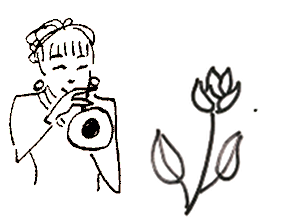
\includegraphics[height=2.5cm]{../figs/ttt.png}};
\end{tikzpicture}
\lfr{Girl playing: \url{http://www.film.queensu.ca/tulips/default.html}}
\end{ftst}

%=====

\begin{ftst}
{Pre-experimental design}
{Definition of hypotheses}
\bitems Exploratory experimentation $\neq$ careless experimentation;
	\spitem Data collection guided by questions of interest;
	\bitems Difference on average/best/worst performance;
		\spitem Robustness / reliability;
	\eitem
	\spitem The translation \textit{scientific question} $\rightarrow$ \textit{test hypothesis} requires special attention, and a solid knowledge of the technical area in which the experiment is being performed;
\eitem
\end{ftst}

%=====

\begin{ftst}
{Choice of Experimental Design}
{Experimental design}
\bitems (Relatively) simple, as long as the pre-experimental part is well done;
	\spitem Dependent on what is being tested (statistical question);
	\spitem A sound design tends to determine the analyses technique to be used, at least  qualitatively;
	\spitem Involves considerations about:
	\bitems Sample size;
		\item Ordering of observations;
		\item Determination of restrictions to the randomization and the use of blocks, etc.
	\eitem
	\spitem Available in several statistical/mathematical packages;
\eitem
\end{ftst}

%=====

\begin{ftst}
{Choice of Experimental Design}
{Problem-dependent}
\bitems Depending on the experimental question, different experimental designs are required
	\spitem A solid, statistically sound design tends to determine which statistical tests must be employed in the analysis step, at least qualitatively.
	\spitem Quantification of the proportion between intra-groups and inter-groups variability;
\eitem
\end{ftst}

\begin{ftst}
{Actual Experiment}
{Data gathering}
\bitems Must be consistent with design, otherwise the validity of the results may be compromised - data collection must always follow the plan:\vhalf
	\bitems No premature stops;	
		\spitem\textit{No-peeking rule}\footnote[1]{Except when planned, of course.};
	\eitem
	\spitem Use of pilot experiments:\vhalf
	\bitems Gathering of preliminary information;
		\spitem Practice with the experimental conditions;
	\eitem
\eitem
\end{ftst}

%=====

\begin{ftst}
{Analysis of the experimental data}
{A consequence of design}
\bitems Analysis techniques are generally relatively simple, but \textit{the devil is in the details};
	\spitem Use of existing statistical tools and frameworks, such as
\eitem
\begin{center}
\includegraphics[width=0.2\textwidth]{../figs/rlogo.png}
\end{center}
\bitems Free, versatile, good graphical capabilities, relatively simple\\
(but with one hell of a learning curve);
\eitem
\end{ftst}

%=====

\begin{ftst}
{Analysis of the experimental data}
{Statistical modeling}
\bitems General procedure for testing the experimental hypotheses:

	\bitems Definition of a \textit{null-model} (absence of effects) and of a desired level of significance;
		\spitem Determination of $P(data|\mbox{\textit{null-model}})$;
		\spitem Decision by rejection (or not) of the null hypothesis;
		\spitem Validation of model assumptions;
		\spitem Estimation of the  \textit{magnitude} of differences - \textbf{practical significance};
	\eitem
\eitem

\begin{block}{}
	\centering\textit{Statistical methods do not \textbf{prove} anything, but they allow an objective definition of margins of plausibility for certain statements.}
\end{block}
\end{ftst}

%=====

\begin{ftst}
{Reporting of results}
{Presentation}
Combine textual, numeric and graphical elements to tell a story with your data. It simplifies the understanding and analysis of the results.
\begin{columns}[T]
\column{0.75\textwidth}
	\bitems Strive to achieve graphical excellence;
		\spitem Coherence of notation - special attention to figures and tables;
		\spitem Display simultaneous confidence intervals and other graphical indicators of effect size.
	\eitem
\column{0.25\textwidth}
	\centering
\includegraphics[height=2.5cm]{../figs/tufte.jpg}\\
	\vone
	\centering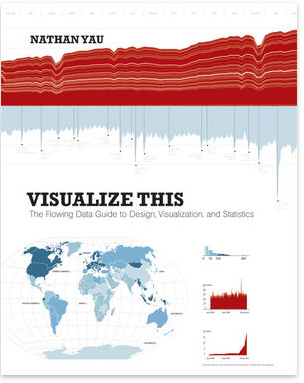
\includegraphics[height=2.5cm]{../figs/yau.png}
\end{columns}
\lfr{Other great resources on graphical excellence:}
\lfr{\textit{Flowing Data} (\url{http://flowingdata.com/})}
\lfr{\textit{Information is Beautiful} (\url{http://www.informationisbeautiful.net})}
\end{ftst}

\begin{ftst}
{Conclusions}
{Drawing and reporting conclusions}
\bitems Conclusions should be based on solid evidence from the data;
	\spitem Be conservative - it is common to exaggerate the generality of the results;
	\spitem Report significance levels and the assumptions under which the results are valid;
	\spitem \textit{Suggest explanations} to the observed results;
	\spitem Careful with \textit{anomaly hunting};
\eitem

\begin{colorblock}{}{bg=green!30,fg=black}
	\small\textit{Always let the science drive the statistics. If you get a statistically significant result, go back and describe what it means in the scientific context.}
	\flushright\small -- Aaron Rendahl
\end{colorblock}
\end{ftst}

\begin{ftst}
{Discussion}
 {Some more relevant points}
\bitems Use of previous knowledge, theoretical or empirical;
	\spitem Iterative experimentation;
	\spitem Statistical $\times$ practical significance;
	\spitem Use of additional experiments to validate conclusions.
\eitem
\end{ftst}



\begin{ftst}
{Bibliography}
{\ }
\scriptsize
\textbf{Required reading}

\benums Dept. Biochemistry \& Cell Biology, Rice University , \textit{Common Errors in Student Research Papers.} - {\tiny\url{http://www.ruf.rice.edu/~bioslabs/tools/report/reporterror.html}}
\item T. Brady, \textit{Reviewer's quick guide to common statistical errors in scientific papers.}\\
{\tiny\url{http://goo.gl/96Qfk}}
\item R.M. Szydloa et al., \textit{Sign of the Zodiac as a predictor of survival for recipients of an allogeneic stem cell transplant for chronic myeloid leukaemia (CML): an artificial association.} Transplantation Proceedings 42 (8):3312-3315, 2010.
\item D.C. Montgomery, \textit{Design and Analysis of Experiments}, Chapter 1. 5th ed., Wiley, 2005
\eenum

\textbf{Recommended reading}

\benums A. Rendahl, \textit{Experimental design and statistical analysis: questions to consider as you write your grant.} - {\tiny\url{http://goo.gl/yT0TK7}}
\item J. Maddox et al., \textit{``High-dilution'' experiments a delusion.} Nature 334, 287-290, 1988
\item V. Czitron, \textit{One-Factor-at-a-Time Versus Designed Experiments.} The American Statistician, 53(2) 126-131, 1999.
\item B. Dunning, \textit{An Enthusiast's Primer on Study Types}. Skeptoid Podcast, Skeptoid Media, Inc., 2013. - 
{\tiny\url{http://skeptoid.com/episodes/4381}}

\eenum
\end{ftst}

%=====

\begin{ftstf}{About this material}{Conditions of use and referencing}
\centering\footnotesize This work is licensed under the Creative Commons CC BY-NC-SA 4.0 license\\(Attribution Non-Commercial Share Alike International License version 4.0).\\
\vhalf
\url{http://creativecommons.org/licenses/by-nc-sa/4.0/}\\
\vone
\footnotesize Please reference this work as:\\
\footnotesize \flushleft Felipe Campelo (2015), \textit{Lecture Notes on Design and Analysis of Experiments}.\\Online: {\scriptsize\url{https://github.com/fcampelo/Design-and-Analysis-of-Experiments}}\\
Version 2.11, Chapter 2; Creative Commons BY-NC-SA 4.0.\\

\begin{Verbatim}[fontsize=\tiny]
    @Misc{Campelo2015-01,
      title={Lecture Notes on Design and Analysis of Experiments},
      author={Felipe Campelo},
      howPublished={\url{https://github.com/fcampelo/Design-and-Analysis-of-Experiments}},
      year={2015},
      note={Version 2.11, Chapter 2; Creative Commons BY-NC-SA 4.0.},
    }
\end{Verbatim}

\begin{tikzpicture} [remember picture,overlay]
\node[anchor=south,yshift=0pt] at (current page.south){ \includegraphics[width=.2\textwidth]{../figs/CCSomerights.png}};
\end{tikzpicture}
\end{ftstf}


\end{document}